% =====================================================================================================
% AURORA / CASSANDRA -- Final Technical Report (IASTAM 6.0, Track 5, Problem 10)
% Build:  pdflatex final_report && bibtex final_report && pdflatex final_report && pdflatex final_report
% Every number in this report comes from a file under results/ or docs/NUMBERS.md in the repository
% (branch p9-integration), produced by the command named next to it. Nothing is a flight measurement.
% =====================================================================================================
\documentclass[conference]{IEEEtran}

\usepackage[T1]{fontenc}
\usepackage{amsmath}
\usepackage{amssymb}
\usepackage{graphicx}
\usepackage{booktabs}
\usepackage{multirow}
\usepackage{array}
\usepackage{xcolor}
\usepackage{url}
\usepackage{cite}
\usepackage{tikz}
\usetikzlibrary{positioning,arrows.meta,fit,backgrounds,calc,shapes.misc}
\usepackage{pgfplots}
\pgfplotsset{compat=1.16}
\usepackage[ruled,vlined,linesnumbered]{algorithm2e}

\newcommand{\file}[1]{\texttt{#1}}
\newcommand{\Pf}[1]{P\!\left(F < t+#1\right)}
\newcommand{\degC}{$^{\circ}$C}
\newcommand{\Jcost}{\mathcal{J}}

\begin{document}

\title{CASSANDRA: Forecasting Mission Failure Before It Happens --\\
A Physics-Constrained, Twin-in-the-Loop Cyber Defence\\for a Hybrid Satellite Constellation Testbed}

\author{
\IEEEauthorblockN{Mayssam Hergli, Youssef Mhamdi, Rami Troudi, Eya Jendoubi, Youssef Atig}
\IEEEauthorblockA{National Institute of Applied Science and Technology (INSAT), Tunis, Tunisia\\
IASTAM 6.0 Technical Challenge --- Track 5 (Cybersecurity), Problem 10:\\
``Detecting an Attack Before Mission Failure''}
}

\maketitle

% -----------------------------------------------------------------------------------------------------
\begin{abstract}
Attacks on space systems unfold in stages: a malicious telecommand or a compromised neighbour drives a
satellite towards a physical failure long before any single-parameter limit trips. We present
CASSANDRA, a predictive defence that asks \emph{how long remains until mission failure} and responds
before it. CASSANDRA ingests telemetry, telecommand provenance and inter-satellite link state;
forecasts the probability of reaching a critical state within 10--120\,s with a calibrated
five-member temporal graph network whose messages may only travel along engineering, threat and
feasible-link relations; checks cross-channel physical consistency to expose masked telemetry; and
chooses the least disruptive response by rolling candidate actions forward on a shadow digital twin
under an explicit cost $\Jcost(a)$, guarded by an uncertainty gate and an isolation budget. It runs on
AURORA, a 12-satellite testbed in which a digital twin and a physical ESP8266 node speak the same MQTT
contract. On held-out out-of-distribution synthetic scenarios, at a 0.1\,\% false-positive rate, the
forecaster warned of all 113 failures (95\,\% Wilson interval 96.7--100\,\%) with a median lead of
135\,s, against 56\,s for a static threshold and 23\,s for trajectory extrapolation; ensemble inference
takes 17.6\,ms per tick on a laptop CPU. In closed loop, 13 of 18 failures were averted (an upper
bound: the planner uses the simulator as its model). Heater-latch, telemetry-masking and cross-link
propagation attacks were contained before any limit in the recorded live runs, including an attack on
the physical node (firmware-emulated temperature) stopped at 54.4\,\degC{} against a 60\,\degC{}
limit. All results are simulated or emulated; we report the limits, including a saturated benchmark.
\end{abstract}

\begin{IEEEkeywords}
Satellite cybersecurity, failure forecasting, temporal graph neural networks, digital twin,
intrusion response, SPARTA.
\end{IEEEkeywords}

% =====================================================================================================
\section{Introduction and Problem Formulation}
\label{sec:intro}

\subsection{Context}
The 2022 attack on the KA-SAT network used a compromised management segment to push a wiper to tens of
thousands of user terminals~\cite{viasat2022,acidrain2022}; the chain unfolded in stages, and the
early signals were weak and spread across components. On board a spacecraft the same pattern appears
as an odd command, a small thermal drift or a slight attitude perturbation, each harmless on its own.
Limit checking on single parameters, the backbone of satellite fault management, fires only once the
physical damage is under way.

Problem~10 of the IASTAM~6.0 Technical Challenge asks for a mechanism that detects malicious or
abnormal behaviour across commands, telemetry, network activity and software behaviour \emph{without
interrupting the mission}, evaluated on detection rate, false positives, detection time, robustness and
availability impact. Our answer replaces the question ``is this value abnormal now?'' with ``where is
this attack going, and how long until the mission fails?'', and acts before the critical point with the
least disruptive response. The defence loop has six stages: \emph{Observe, Understand, Forecast,
Simulate, Act, Verify}.

\subsection{System model}
Let $\mathcal{S}=\{A,\dots,L\}$ be a constellation of $|\mathcal{S}|=12$ satellites observed in ticks
of $\Delta t = 1$\,s. At tick $t$, satellite $s$ downlinks a telemetry vector $\mathbf{y}_s(t)$
(thermal, power, attitude, on-board computer, communications and sun-sensor fields), receives
telecommands $\mathcal{C}_s(t)$, each tagged with an origin $o \in \{\textit{ground},
\textit{core}, \textit{isl}{:}x, \textit{unknown}\}$, and maintains inter-satellite links
$\ell_{ij}(t) = \mathrm{feas}_{ij}(t) \wedge \mathrm{en}_{ij}(t)$, where feasibility comes from
geometry (line of sight and range) and the enable flags from commands.

\subsection{Critical state}
Following the interim paper, mission failure of satellite $s$ is the first time
\begin{equation}
F_s(t) = \big(|\theta^{\mathrm{err}}_s| > \theta^{\max}_s\big)\ \vee\
\big(\mathrm{SOC}_s < \mathrm{SOC}^{\min}_s\big)\ \vee\ \big(T^{\mathrm{bus}}_s > T^{\max}_s\big)
\label{eq:F}
\end{equation}
holds, with per-satellite limits (Table~\ref{tab:limits}). We write $\tau^F_s$ for the critical time
when responses are disabled.

\begin{table}[t]
\caption{Critical-state limits per satellite kind (\file{docs/interfaces.md}, Sec.~5).}
\label{tab:limits}
\centering
\begin{tabular}{@{}lccc@{}}
\toprule
Satellite kind & $T^{\max}$ & $\mathrm{SOC}^{\min}$ & $\theta^{\max}$ \\
\midrule
Digital-twin satellite (default) & 45\,\degC & 30\,\% & 10$^{\circ}$ \\
ESP8266 node (emulated temperature) & 60\,\degC & n/a & n/a \\
\bottomrule
\end{tabular}
\end{table}

\subsection{Problem statement}
From the observable history $\mathcal{H}(t)$ (telemetry, telecommands with origins, link state; never
ground-truth labels), the defence must, for every satellite and horizon
$\Delta\in\mathcal{D}=\{10,30,60,120\}$\,s, estimate the hazard
\begin{equation}
p_s(t,\Delta) = \Pr\big(t < \tau^F_s \le t+\Delta \;\big|\; \mathcal{H}(t)\big),
\label{eq:hazard-goal}
\end{equation}
raise an alert at the first tick where $p_s(t,\Delta^\star)\ge\tau$, and choose an action
$a(t)\in\mathcal{A}$ that minimises expected failures while preserving service. The operating
objective is
\begin{equation}
\max_{\tau}\ \mathbb{E}\big[\tau^F_s - T^{\mathrm{alert}}_s\big]
\quad \text{s.t.}\quad \mathrm{FPR}(\tau)\le 10^{-3},
\label{eq:objective}
\end{equation}
where the false-positive rate is measured on benign (clean and natural-fault) timesteps.

\subsection{Operational constraints}
\begin{itemize}
\item \textbf{Latency:} one decision per 1\,s tick; inference plus planning within a 150\,ms budget.
\item \textbf{Dynamic links:} responses may reroute only over links that are geometrically feasible
at that time; quarantine physically disables a node's links.
\item \textbf{Power and thermal:} the critical state (\ref{eq:F}) bounds battery state of charge and
bus temperature; safe mode sheds the heater and non-essential loads.
\item \textbf{Bandwidth:} the full constellation produces 72 telemetry and 66 link messages per second
at 1\,Hz (Sec.~\ref{sec:impl}).
\item \textbf{Anti-self-denial-of-service:} an attacker may fake precursors to make the defence
isolate healthy satellites, so autonomous isolation is limited (Sec.~\ref{sec:safety}).
\end{itemize}

\subsection{Contributions}
\begin{enumerate}
\item A calibrated, physics-constrained temporal graph forecaster of time-to-failure with an explicit
0.1\,\% false-positive operating point and an ensemble uncertainty used by a safety gate.
\item A twin-in-the-loop response planner that scores candidate actions with
$\Jcost(a)$ on a shadow model that never sees the attacker's queued commands.
\item A cross-channel consistency monitor, bounded by the design thermal model, that exposes masked
telemetry.
\item AURORA, a hybrid hardware/digital-twin testbed with a frozen message contract, ground-truth
isolation enforced by tests, and an evaluation protocol that reports pre-onset false alarms and labels
upper bounds.
\end{enumerate}

% =====================================================================================================
\section{Related Work}
\label{sec:related}

\textbf{Telemetry anomaly detection.} Spacecraft operations rely on static limits; data-driven
detectors such as LSTM forecasting with dynamic thresholds~\cite{hundman2018telemanom} and LSTM
autoencoders~\cite{malhotra2016lstmed} score how unusual the present is. Graph Deviation
Networks~\cite{deng2021gdn} learn a sensor graph and score forecast deviations. Benchmarks with real
operational telemetry exist (ESA-ADB~\cite{esaadb}, OPS-SAT-AD~\cite{opssatad}). These methods output
an anomaly score, not a time to a mission-level critical state, and do not separate an attack from a
fault.

\textbf{Space cyber threat modelling and data.} SPARTA~\cite{sparta} catalogues space-specific
techniques and countermeasures; a secure-by-component decomposition~\cite{benyahia2024} gives the
engineering dependencies an attack must travel through. Labelled cyber datasets are scarce: SCAD
(FireSat digital twin, reaction-wheel override attacks)~\cite{scad} and CuCD-ID (NOS3/cFS)~\cite{cucdid}.
Our team's analysis of SCAD (225 attack runs against matched baselines, \file{eval/datasets/scad.py})
showed an ordered cascade --- actuators at once, attitude and sun sensors after about 20--30\,s, star
tracker and power after about 2\,min --- which motivates forecasting the \emph{next affected
subsystem}.

\textbf{Temporal graph learning and uncertainty.} Temporal graph networks~\cite{rossi2020tgn} combine
per-node memory with message passing; relational~\cite{schlichtkrull2018rgcn} and
attention~\cite{velickovic2018gat} layers handle typed edges. Temperature scaling~\cite{guo2017calibration}
and deep ensembles~\cite{lakshminarayanan2017ensembles} provide calibration and uncertainty.

\textbf{Testbeds.} Satellite security testbeds such as AegisSat~\cite{aegissat} and
MimicSat~\cite{mimicsat} emulate the flight software or the cyber-physical plant.

\textbf{Gap and our added value.} We found no system that (i) forecasts a calibrated probability of
mission failure per horizon from cyber and physical evidence together, (ii) restricts learning to
physically permitted propagation paths, (iii) selects a response by counterfactual simulation under
explicit anti-self-DoS gates, and (iv) is evaluated with a fixed false-positive operating point,
held-out generator families and closed-loop availability. CASSANDRA addresses all four, and its
evaluation reports where the evidence is still weak (Sec.~\ref{sec:feas}).

% =====================================================================================================
\section{System Architecture and Technical Specifications}
\label{sec:arch}

\subsection{Decomposition}
AURORA (Fig.~\ref{fig:arch}) has five parts connected by one MQTT~\cite{mqtt5} bus
(Mosquitto~\cite{light2017mosquitto}, ports 1883 and 9001 for WebSockets):
\begin{itemize}
\item \textbf{Space segment:} a digital twin (\file{twin/service.py}) running the 12-satellite physics
of \file{ml/synthetic/engine.py} at 1\,Hz, and a physical NodeMCU ESP8266 node playing satellite~B
through a serial-to-MQTT bridge (\file{hardware/esp8266\_bridge}). Both publish the same messages;
the twin marks them \texttt{src:"twin"}, the node \texttt{src:"hw"} with
\texttt{emulated:["temp\_c"]}.
\item \textbf{CASSANDRA core} (\file{cassandra/}): ingest, monitor, forecast, sandbox, act, explain,
incident correlator; one pass per tick of message time.
\item \textbf{Red team} (\file{attacks/run.py}): attacks A1, B1, C1, faults and clean runs; ground
truth goes only to \texttt{gt/}.
\item \textbf{Recorder} (\file{twin/recorder.py}): the scorer, the only process that reads
ground truth.
\item \textbf{Operator dashboard} (\file{dashboard/}): single page over WebSockets, read-only.
\end{itemize}

\begin{figure*}[t]
\centering
\resizebox{\textwidth}{!}{%
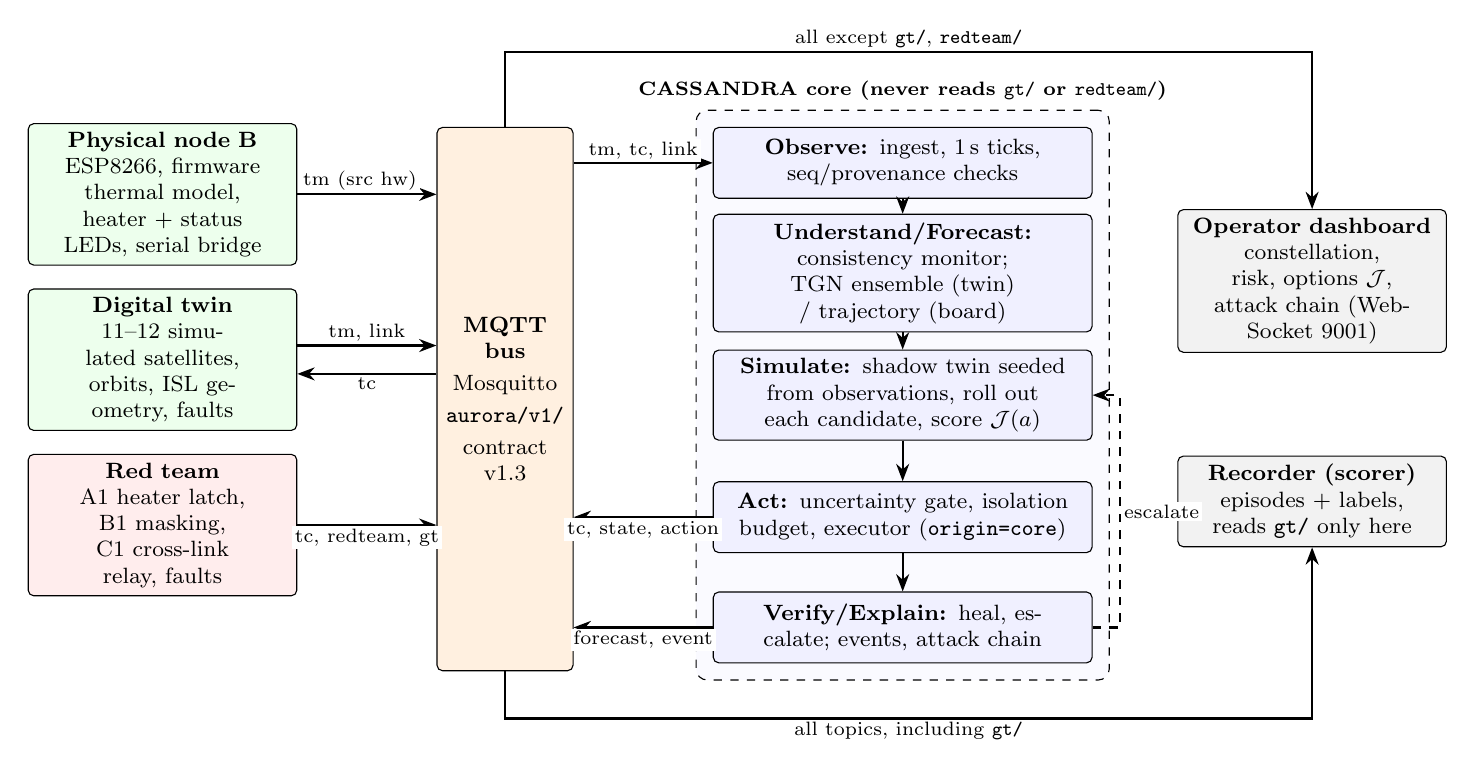
\begin{tikzpicture}[
  font=\footnotesize, >={Stealth[length=2.2mm]},
  box/.style={draw, rounded corners=2pt, align=center, inner sep=3pt, minimum height=9mm},
  plant/.style={box, fill=green!7, text width=32mm},
  stage/.style={box, fill=blue!6, text width=46mm},
  side/.style={box, fill=gray!10, text width=32mm},
  attack/.style={box, fill=red!7, text width=32mm},
  lbl/.style={font=\scriptsize, align=center, fill=white, inner sep=1pt},
  flow/.style={->, thick},
]
% space segment
\node[plant] (board) at (0,3.0) {\textbf{Physical node B}\\ESP8266, firmware thermal model,\\heater + status LEDs, serial bridge};
\node[plant] (twin)  at (0,0.9) {\textbf{Digital twin}\\11--12 simulated satellites,\\orbits, ISL geometry, faults};
\node[attack] (atk)   at (0,-1.2) {\textbf{Red team}\\A1 heater latch, B1 masking,\\C1 cross-link relay, faults};
% bus
\node[draw, fill=orange!12, rounded corners=2pt, minimum width=17mm, minimum height=69mm,
      align=center] (bus) at (4.35,0.4) {\textbf{MQTT}\\\textbf{bus}\\[2pt]Mosquitto\\[2pt]\texttt{aurora/v1/}\\[2pt]contract\\v1.3};
% core
\node[stage] (ing)  at (9.4,3.4)  {\textbf{Observe:} ingest, 1\,s ticks, seq/provenance checks};
\node[stage] (und)  at (9.4,2.0)  {\textbf{Understand/Forecast:} consistency monitor;\\TGN ensemble (twin) / trajectory (board)};
\node[stage] (sim)  at (9.4,0.45) {\textbf{Simulate:} shadow twin seeded from observations, roll out each candidate, score $\mathcal{J}(a)$};
\node[stage] (act)  at (9.4,-1.1) {\textbf{Act:} uncertainty gate, isolation budget, executor (\texttt{origin=core})};
\node[stage] (ver)  at (9.4,-2.5) {\textbf{Verify/Explain:} heal, escalate; events, attack chain};
\begin{scope}[on background layer]
\node[draw, dashed, rounded corners=4pt, fill=blue!2, inner sep=6pt, fit=(ing)(ver),
      label={[font=\scriptsize\bfseries, align=center]above:CASSANDRA core (never reads \texttt{gt/} or \texttt{redteam/})}] (core) {};
\end{scope}
% consumers
\node[side] (dash) at (14.6,1.9)  {\textbf{Operator dashboard}\\constellation, risk, options $\mathcal{J}$,\\attack chain (WebSocket 9001)};
\node[side] (rec)  at (14.6,-0.9) {\textbf{Recorder (scorer)}\\episodes + labels,\\reads \texttt{gt/} only here};
% flows: space segment <-> bus
\draw[flow] (board.east) -- node[lbl, above, pos=0.45]{tm (src hw)} (board.east -| bus.west);
\draw[flow] ($(bus.west |- twin.east)+(0,-0.18)$) -- node[lbl, below, pos=0.5]{tc} ($(twin.east)+(0,-0.18)$);
\draw[flow] ($(twin.east)+(0,0.18)$) -- node[lbl, above, pos=0.5]{tm, link} ($(bus.west |- twin.east)+(0,0.18)$);
\draw[flow] (atk.east) -- node[lbl, below, pos=0.5]{tc, redteam, gt} (atk.east -| bus.west);
% bus <-> core
\draw[flow] (bus.east |- ing.west) -- node[lbl, above]{tm, tc, link} (ing.west);
\draw[flow] (act.west) -- node[lbl, below]{tc, state, action} (bus.east |- act.west);
\draw[flow] (ver.west) -- node[lbl, below]{forecast, event} (bus.east |- ver.west);
% pipeline
\draw[flow] (ing) -- (und);
\draw[flow] (und) -- (sim);
\draw[flow] (sim) -- (act);
\draw[flow] (act) -- (ver);
\draw[flow, dashed] (ver.east) -- ++(0.35,0) |- node[lbl, right, pos=0.25]{escalate} (sim.east);
% bus -> consumers (routed over and under the core)
\draw[flow] (bus.north) -- ++(0,0.95) -| node[lbl, above, pos=0.25]{all except \texttt{gt/}, \texttt{redteam/}} (dash.north);
\draw[flow] (bus.south) -- ++(0,-0.6) -| node[lbl, below, pos=0.25]{all topics, including \texttt{gt/}} (rec.south);
\end{tikzpicture}%
}
\caption{AURORA architecture and the CASSANDRA loop (Observe $\rightarrow$ Understand/Forecast
$\rightarrow$ Simulate $\rightarrow$ Act $\rightarrow$ Verify/Explain). Ground-truth isolation is
enforced by an allow-list of subscriptions and a test (\file{tests/cassandra/test\_gt\_isolation.py}).}
\label{fig:arch}
\end{figure*}

\subsection{Interface contract}
All components meet at one versioned contract (\file{docs/interfaces.md} v1.3, validated by pydantic
models in \file{aurora\_common/}). Table~\ref{tab:topics} lists the topics. Telemetry carries a
per-stream sequence number (gaps are evidence), telecommands a unique id and origin (relays keep the
id), and every payload a schema version. The core subscribes to exactly three filters
(\texttt{sat/+/tm/+}, \texttt{sat/+/tc}, \texttt{link/+}); the bus wrapper refuses any other.

\begin{table}[t]
\caption{Topic tree (prefix \texttt{aurora/v1/}), from \file{docs/interfaces.md}.}
\label{tab:topics}
\centering
\footnotesize
\setlength{\tabcolsep}{3pt}
\begin{tabular}{@{}llc@{}}
\toprule
Topic & Publisher $\rightarrow$ subscribers & QoS \\
\midrule
\texttt{sat/\{id\}/tm/\{sub\}} & node, twin $\rightarrow$ anyone & 0 \\
\texttt{sat/\{id\}/tc} & ground, core, attacker, relay $\rightarrow$ anyone & 1 \\
\texttt{sat/\{id\}/state} & core $\rightarrow$ anyone (retained) & 1 \\
\texttt{link/\{a\}-\{b\}} & twin $\rightarrow$ anyone & 0 \\
\texttt{core/forecast/\{id\}} & core $\rightarrow$ anyone & 0 \\
\texttt{core/action}, \texttt{core/event} & core $\rightarrow$ anyone & 1 \\
\texttt{redteam/\{id\}} & attacker $\rightarrow$ twin, bridge only & 1 \\
\texttt{gt/episode}, \texttt{gt/event} & attacker, twin $\rightarrow$ recorder only & 1 \\
\bottomrule
\end{tabular}
\end{table}

\subsection{Threat scenarios}
Table~\ref{tab:scenarios} maps the three attack scenarios to SPARTA~\cite{sparta} (technique mapping
refined in Phase~3). Natural faults (sensor drift, single-event upset, battery ageing, eclipse entry,
stuck heater) must not be confused with attacks. We assume the adversary cannot falsify every
independent measurement channel of a subsystem at once.

\begin{table}[t]
\caption{Attack scenarios and SPARTA mapping (\file{docs/interfaces.md}, Sec.~7).}
\label{tab:scenarios}
\centering
\footnotesize
\setlength{\tabcolsep}{3pt}
\begin{tabular}{@{}p{8mm}p{36mm}p{30mm}@{}}
\toprule
ID & Mechanism & SPARTA \\
\midrule
A1 & Latched ground \texttt{HEATER on} drives $T^{\mathrm{bus}}$ to its limit & IA-0009 Trusted Relationship \\
B1 & Reported \texttt{temp\_c} frozen while the heater runs & DE-0002 Disrupt/Deceive Downlink \\
B2 & Slow bias on a reported channel & DE-0003 On-Board Values Obfuscation \\
C1 & Compromised satellite relays the attack to neighbours over ISLs & IA-0003 Crosslink via Compromised Neighbor \\
\bottomrule
\end{tabular}
\end{table}

\subsection{Responses and states}
Candidate actions are $\mathcal{A}=\{\textit{none}, \textit{safe\_mode}, \textit{block\_source},
\textit{isolate\_subsystem}, \textit{quarantine}\}$: switching the heater off, disabling the links to a
relaying origin, safe mode (heater off, non-essential loads off, only ground and core commands
accepted), and quarantine (safe mode plus disabling every link of the node, rerouting only over
feasible links). They operationalise the SPARTA countermeasures CM0032 (on-board intrusion detection),
CM0042 (robust fault management: contain, observe, heal) and CM0070 (alternate communication paths).
Each satellite moves through the states \emph{nominal}, \emph{flagged}, \emph{quarantined} or
\emph{safe\_hold}, and back to \emph{nominal} when healed.

% =====================================================================================================
\section{Methodology and Mathematical Formulation}
\label{sec:method}

\subsection{Typed cyber-physical graph}
At each tick we build $G_t=(V,E_t,X_t)$. Nodes are the six subsystems of every satellite plus one node
per satellite. Edges are typed: engineering dependencies $E_{\mathrm{eng}}$ (e.g.\
heater$\rightarrow$temperature$\rightarrow$battery, wheels$\rightarrow$attitude$\rightarrow$solar
power), SPARTA attack relations $E_{\mathrm{sp}}$, aggregation edges (subsystem$\rightarrow$satellite)
and the inter-satellite links that exist at time $t$, $E_{\mathrm{isl}}(t)=\{(i,j):\ell_{ij}(t)\}$.
Learned couplings exist only as attributes of permitted edges. Each satellite contributes 27 channels
per tick: the telemetry fields, first differences, counter increments and telecommand counts per origin
(\textit{ground}, \textit{isl}, \textit{unknown}) and type; the 12 satellites share 66 link states.

\textbf{Physical residual.} For each engineering edge $(i\!\rightarrow\! j)$ a ridge model $g_{ij}$
fitted on nominal data predicts the change of $j$ from $i$; the residual
\begin{equation}
\Delta\Phi_{ij}(t) = \big|\,\Delta x_j(t) - g_{ij}\big(x_i(t-k{:}t)\big)\big|
\label{eq:residual}
\end{equation}
separates benign operations, whose effects the engineering model explains, from induced effects.

\subsection{Learned forecaster}
For a 30\,s window, a GRU~\cite{cho2014gru} per node encodes the node's history and a small GRU per
engineering edge encodes its residual sequence. Three rounds of relation-aware message passing follow,
with one weight matrix per relation~\cite{schlichtkrull2018rgcn} and attention over incoming
edges~\cite{velickovic2018gat}:
\begin{equation}
\mathbf{h}^{(l+1)}_v = \sigma\Big(W_0\mathbf{h}^{(l)}_v + \sum_{r}\sum_{u\in\mathcal{N}_r(v)}
\alpha^{(l)}_{uv}\, m_{uv}(t)\, W_r \mathbf{h}^{(l)}_u\Big),
\label{eq:mp}
\end{equation}
where $m_{uv}(t)=\ell_{uv}(t)$ for ISL edges and 1 otherwise, so a message crosses only a feasible,
enabled link. A test asserts that with every ISL disabled, perturbing one satellite cannot change
another's forecast.

\textbf{Discrete-time hazard head.} With one logit $b_k$ per horizon bin and $\Delta_1<\dots<\Delta_4$,
\begin{equation}
\hat p(t,\Delta_k) = 1-\prod_{j\le k}\big(1-\sigma(b_j/T)\big),
\label{eq:hazard}
\end{equation}
which is monotone in the horizon by construction; $T$ is the calibration temperature. Two more heads
predict the next affected subsystem (softmax over six) and $P(\text{malicious}\mid\text{anomaly})$.

\textbf{Loss with censoring.} With hazard targets $y_{k}=\mathbf{1}[t<\tau^F\le t+\Delta_k]$ and a mask
$m_k$ that removes windows after failure and right-censored windows (a satellite at risk whose episode
ends before $t+\Delta_k$),
\begin{equation}
\mathcal{L} = \frac{\sum_k m_k\,\mathrm{BCE}_{w^+}(\hat p_k, y_k)}{\sum_k m_k}
+ 0.3\,\mathrm{CE}(\hat{\mathbf{q}}, \mathrm{next}) + 0.3\,\mathrm{BCE}(\hat\mu, \mathrm{mal}),
\label{eq:loss}
\end{equation}
with positive weight $w^+=3$. Training samples half of its windows uniformly and half around the
anomaly.

\textbf{Calibration, ensemble and alert level.} The temperature $T$ minimises the masked negative
log-likelihood of (\ref{eq:hazard}) on validation windows~\cite{guo2017calibration}. Five members
$m=1..5$ trained from different seeds~\cite{lakshminarayanan2017ensembles} give
\begin{equation}
\bar p = \frac{1}{5}\sum_{m}\hat p^{(m)},\qquad
Q = \sqrt{\frac{1}{5}\sum_m \big(\hat p^{(m)}-\bar p\big)^2}\ \ \text{at } \Delta^\star=60\,\mathrm{s}.
\label{eq:ensemble}
\end{equation}
$Q$ is a standard deviation, not a variance, because the variance of a probability is at most $0.25$
and could never exceed the gate threshold $0.35$. The alert level $\tau$ is the $(1-10^{-3})$ quantile
of $\bar p(t,60)$ over benign validation timesteps; with the deployed models $T=0.730$ and
$\tau=0.0153$ (\file{data/models/calibration.json}, release \texttt{models-v2}).

\subsection{Trajectory forecaster (physical node)}
On the physical node, whose telemetry differs from the training distribution, the core uses the Phase~2
predictor, generalised. For each limited channel $x$ with limit $L$ and sign $\sigma_x$, a Theil--Sen
slope~\cite{sen1968theilsen} $\dot x$ over the last $w$ ticks gives
\begin{equation}
t_c = \frac{\sigma_x (L-x)}{\sigma_x\dot x},\qquad
\hat p(t,\Delta)=\max_x\ \mathrm{clip}\Big(1-\frac{t_c}{\Delta},0,1\Big),
\label{eq:traj}
\end{equation}
with $\hat p=0$ when the channel is not approaching its limit. The median of pairwise slopes makes a
single-tick upset (fault F2) harmless. This forecaster predicts neither the next subsystem nor
maliciousness, so it publishes \texttt{null} for them; a channel enters (\ref{eq:traj}) only after a
full window of real readings, so a node that does not report a subsystem never raises a false alarm.

\subsection{Cross-channel consistency monitor}
Each twin satellite has a design thermal model
\begin{equation}
C\,\frac{dT}{dt} = P_{\mathrm{heater}} + \alpha P_{\mathrm{sun}}(1-e) + P_{\mathrm{int}}
- k\,(T-T_{\mathrm{env}}),
\label{eq:thermal}
\end{equation}
with $C=300$\,J/K, $k=2$\,W/K, $T_{\mathrm{env}}=-10$\,\degC{} and a commanded heater between 50 and
90\,W. From it we derive, at temperature $T$, the slowest plausible rise $r_{\min}(T)$ (weakest
heater, eclipse) and the fastest $r_{\max}(T)$. With the heater on for the whole 10\,s window, the
rule
\begin{equation}
\hat{\dot T} + 2\,\mathrm{SE}(\hat{\dot T}) < r_{\min}(T)
\label{eq:monitor}
\end{equation}
flags the reported temperature as inconsistent; a reading identical over the window is flagged as
frozen. A hit marks \texttt{temp\_c} untrusted; the forecaster then estimates the temperature as the
last trusted value plus heater on-time $\times\, r_{\max}(T)$ (conservative: it errs early) until 10
consistent ticks restore trust. Near equilibrium $r_{\min}\approx 0$ and the rule abstains.

\subsection{Counterfactual response selection}
When a flagged satellite reaches $\bar p(t,60)\ge 0.5$, the sandbox builds a shadow
\texttt{SyntheticTwin} seeded from the latest \emph{observations} (temperatures, state of charge,
modes, heater flags, link enable and feasibility, orbit phase) with an \emph{empty} command queue: the
attacker's future commands are never copied. The threat assumption is that observed effects persist
(a latched heater stays on) and that a hazardous command seen at least twice from one origin keeps
arriving at its observed period. Each candidate $a$ is applied and rolled forward for 60\,s, then scored
\begin{equation}
\Jcost(a) = w_r\,R(a) + w_m\big(1-U(a)\big) + w_c\,C(a) + w_q\,Q,
\label{eq:J}
\end{equation}
\begin{equation}
R(a)=\sum_{s\in\mathcal{S}} \max\!\Big(\hat p_s\big(t_a,120\big),\
\mathbf{1}[\text{limit crossed}],\ \rho\,\mathbf{1}[s\in\mathcal{V}_a]\Big),
\label{eq:R}
\end{equation}
where $R$ is the expected number of satellites reaching $F$ (a sum, not a maximum, so actions that
spare more satellites score lower), $\mathcal{V}_a$ the satellites that a continuing relay would newly
reach on the predicted link geometry if $a$ does not stop it ($\rho=1$), $U$ the fraction of satellites
in service and $C$ the cost of the action (Table~\ref{tab:params}). When $Q$ is unavailable (a single
model) its term is dropped rather than set to zero. ``None'' is a candidate, so $\Jcost$ decides whether
acting is worth it. Algorithm~\ref{alg:sandbox} gives the procedure.

\begin{algorithm}[t]
\caption{Sandbox ranking of candidate responses}
\label{alg:sandbox}
\DontPrintSemicolon
\KwIn{world tick $W_t$, target $x$, threats $\Theta$, candidates $\mathcal{A}$, budget state $B$}
\KwOut{candidates ranked by $\Jcost$}
$\mathcal{T} \leftarrow$ \textsc{SeedFromObservation}$(W_t)$ \tcp*{empty queue}
\ForEach{$a \in \mathcal{A}$}{
  \If{$a=\textit{quarantine}$ \textbf{and} $B$ exhausted}{\textbf{continue}\;}
  $\mathcal{T}_a \leftarrow$ copy of $\mathcal{T}$; apply the commands of $a$ (origin \textit{core})\;
  \For{$k\leftarrow 1$ \KwTo $60$}{
    replay each continuing threat in $\Theta$ due at $k$, over feasible enabled links only\;
    step $\mathcal{T}_a$ by 1\,s; mark any satellite whose limit is crossed\;
  }
  $R \leftarrow$ Eq.~(\ref{eq:R}); $U \leftarrow$ fraction in service\;
  $\Jcost(a) \leftarrow w_r R + w_m(1-U) + w_c C(a) + [Q\neq\varnothing]\,w_q Q$\;
}
\Return{$\mathcal{A}$ sorted by $\Jcost$}
\end{algorithm}

\subsection{Safety gates, escalation and healing}
\label{sec:safety}
The best candidate passes two gates before execution. (i)~\emph{Uncertainty gate:} if $Q>0.35$ the core
does not isolate; it enters safe hold and alerts the ground. If $Q$ is unavailable the gate is reported
as inactive, never as passed. (ii)~\emph{Isolation budget:} quarantine is offered only while at most
25\,\% of the constellation (3 of 12) has been quarantined in the current orbital-period window. A
containment that leaves $\bar p\ge 0.5$ for 20\,s, or a heater switched on again more than 2\,s after
the action, escalates along the ladder isolate/block $\rightarrow$ safe mode $\rightarrow$ quarantine;
quarantine of a satellite requires an observed cyber cause. A satellite heals when its temperature is
trusted and below 30\,\degC{} and $\bar p<0.10$ for 3 consecutive ticks, once any continuing threat has
been quiet for twice its period plus 5\,s; healing re-enables the links the core cut and sends
\texttt{SET\_MODE NOMINAL}. Algorithm~\ref{alg:loop} summarises one tick.

\begin{algorithm}[t]
\caption{One CASSANDRA tick (message time)}
\label{alg:loop}
\DontPrintSemicolon
\KwIn{messages of tick $t$ (allow-listed topics only)}
$W_t \leftarrow$ \textsc{Ingest} (hold $\le$3\,s, seq and provenance checks)\;
\ForEach{satellite $s$}{
  $h_s \leftarrow$ \textsc{Monitor}$(W_t, s)$ \tcp*{Eq.~(\ref{eq:monitor})}
  $\hat p_s, Q_s \leftarrow$ \textsc{Forecast}$(W_t, s, h_s)$ \tcp*{Eqs.~(\ref{eq:hazard}),(\ref{eq:traj})}
  \lIf{nominal \textbf{and} ($\hat p_s(60)\ge\tau_s$ \textbf{or} $h_s$)}{state $\leftarrow$ flagged}
  \If{flagged \textbf{and} $\hat p_s(60)\ge 0.5$ \textbf{and} not planned in the last 5\,s}{
    $a^\star \leftarrow$ first of Alg.~\ref{alg:sandbox} that passes the gates\;
    execute $a^\star$; publish action with $\Jcost$ and alternatives\;
  }
  \textsc{Verify}$(s)$: escalate or heal\;
}
\textsc{Explain}: publish forecasts, events and the attack chain\;
\end{algorithm}

\begin{table}[t]
\caption{Decision parameters (\file{cassandra/config.yaml}).}
\label{tab:params}
\centering
\footnotesize
\setlength{\tabcolsep}{4pt}
\begin{tabular}{@{}lr@{}}
\toprule
Parameter & Value \\
\midrule
Weights $(w_r, w_m, w_c, w_q)$ & (1.0, 0.5, 0.3, 0.5) \\
Cost $C$: none / block / safe / isolate / quarantine & 0 / 0.1 / 0.2 / 0.25 / 0.4 \\
Rollout / risk horizon & 60\,s / 120\,s \\
Flag / plan / calm thresholds, $\bar p(t,60)$ & $\tau$ (0.30 traj.) / 0.50 / 0.10 \\
Physical node rule & $\hat p(t,30)\ge 0.85$ \\
Uncertainty gate $\theta$ on $Q$ & 0.35 \\
Isolation budget per orbital window & 25\,\% \\
Escalation after & 20\,s \\
\bottomrule
\end{tabular}
\end{table}

\subsection{Incident correlator}
The correlator (\file{cassandra/incident.py}) assembles an attack chain from observed evidence only:
telecommand origins, monitor hits, forecasts and the core's own actions. Evidence is grouped by satellite
and time window, and across satellites when hazardous commands share an ISL origin. Each step is
labelled \emph{observed} or \emph{predicted}; predicted steps (next subsystem, projected failure) are
refreshed rather than stacked. A risk flag or a hazardous ground command alone opens no incident,
because legitimate heater tests use the same command every orbit.

% =====================================================================================================
\section{Prototype Implementation and Experimental Setup}
\label{sec:impl}

\subsection{Software and hardware stack}
Table~\ref{tab:stack} lists the components. Everything runs on a single laptop (Windows~11 with WSL
Ubuntu, Python~3.11.17, PyTorch~2.14 CPU); the target ground station is a Raspberry~Pi, on which
latency has not yet been measured. The physical node is a NodeMCU ESP8266 (Amica) with three
dual-colour LEDs showing the states of satellites A, B and C; its firmware emulates the bus temperature
(25\,\degC{} ambient, $+1.5$\,\degC/s while the heater is latched) and reports at 2\,Hz over serial to a
self-contained bridge.

\begin{table}[t]
\caption{Repository map (branch \texttt{p9-integration}).}
\label{tab:stack}
\centering
\footnotesize
\setlength{\tabcolsep}{3pt}
\begin{tabular}{@{}p{22mm}p{58mm}@{}}
\toprule
Path & Role \\
\midrule
\file{aurora\_common/} & contract models, topic builders, bus wrapper with allow-list \\
\file{ground/} & Mosquitto (1883 MQTT, 9001 WebSocket) \\
\file{twin/} & live twin service, episode recorder \\
\file{ml/} & synthetic engine, graph, forecaster, training, calibration, baselines, export \\
\file{cassandra/} & core: ingest, monitor, forecast, sandbox, act, explain, incident \\
\file{attacks/} & A1 (\texttt{--reassert}), B1, C1, F1, N over the bus \\
\file{eval/} & harness, metrics, closed loop, robustness, stress, dataset loaders \\
\file{hardware/} & ESP8266 serial-to-MQTT bridge, bring-up guide \\
\file{dashboard/} & operator screen (vendored mqtt.js, uPlot) \\
\bottomrule
\end{tabular}
\end{table}

\subsection{Digital twin and constellation}
The twin integrates thermal (\ref{eq:thermal}), power
($\mathrm{SOC}'=(\eta P_{\mathrm{solar}}\cos\theta(1-e)-P_{\mathrm{load}})/E_{\mathrm{cap}}$, 20\,Wh)
and attitude models (reaction wheels saturating at 6000\,rpm) at 1\,s steps, plus an on-board computer
mode machine and command counters. Twelve satellites fly circular 550\,km orbits in 3 planes of 4
(53$^{\circ}$ inclination); a link is feasible when the line of sight clears the Earth by 100\,km and the
range is at most 5000\,km; eclipse uses a cylindrical shadow; ground contact requires 10$^{\circ}$
elevation over Tunis. Orbit time may be compressed (factor 8) while subsystem physics stays at 1\,s.
At 1\,Hz the full constellation puts $12\times6=72$ telemetry and 66 link messages per second on the bus, as observed on the live twin.

\subsection{Datasets}
The generator (\file{ml/synthetic/}) produces 600\,s episodes of 12 satellites mixing clean
operations (18\,\%), five natural faults (6\,\% each) and attacks A1--A3, B1, B2 and C1, each with
per-satellite truth: onset, critical time, rule, malicious flag and the first time each subsystem
departs from a counterfactual run without the anomaly. Table~\ref{tab:data} gives the splits.
\texttt{test\_ood} holds out whole generator families (pulsed drift, Student-$t$ noise, lower
intensity); \texttt{test\_real} replaces synthetic noise with real residuals and gaps from
OPS-SAT-AD~\cite{opssatad}.

\begin{table}[t]
\caption{Episode splits and model configuration (\file{results/manifest.json}).}
\label{tab:data}
\centering
\footnotesize
\setlength{\tabcolsep}{3pt}
\begin{tabular}{@{}lr@{}}
\toprule
Train / validation episodes & 800 / 200 \\
Test: in-distribution / out-of-distribution / real noise & 300 / 300 / 200 \\
Window, horizons & 30\,s; 10, 30, 60, 120\,s \\
Hidden size, message-passing rounds & 32, 3 \\
Parameters per member (\file{docs/ML\_GUIDE.md}) & 42.7\,k \\
Ensemble seeds; epochs; learning rate & 0--4; 8; $2\times10^{-3}$ \\
Ablations & no eng.\ features, unconstrained, no residual \\
Wall time: train / evaluate & 21\,min / 19\,min \\
\bottomrule
\end{tabular}
\end{table}

\subsection{Baselines and metrics}
Baselines run through the same harness: static thresholds, the Phase~2 trajectory forecaster, an LSTM
autoencoder~\cite{malhotra2016lstmed} and GDN~\cite{deng2021gdn}, plus the ablations. Every method is
scored every 2\,s from tick~0 on the same truth-independent schedule. For each method $\tau$ is chosen
on validation benign timesteps for $\mathrm{FPR}=0.1\,\%$ and applied unchanged to the test splits.
$T^{\mathrm{alert}}$ is the first tick with score $\ge\tau$; an alert before the episode's attack onset is
counted as a false alarm (``pre-onset'') and earns no lead time; lead is
$T^{\mathrm{lead}}=\tau^F-T^{\mathrm{alert}}$, and alerts at or after $\tau^F$ are misses. We report
recall with Wilson intervals~\cite{wilson1927}, median lead with IQR and bootstrap
intervals~\cite{efron1979bootstrap}, expected calibration error (10 bins), next-subsystem accuracy and
the attack-versus-fault AUROC.

\subsection{Execution pipeline}
The results are reproducible from the repository:
\texttt{make models} (download the released ensemble, SHA-256 checked) or
\texttt{python -m ml.synthetic.generate}, \texttt{ml.features}, \texttt{ml.train all},
\texttt{eval.harness run}, \texttt{eval.closed\_loop --episodes 24}, \texttt{eval.robustness},
\texttt{eval.stress}, \texttt{ml.export}; live scenarios with \texttt{make demo-sw} and
\texttt{make attack A1 TARGET=E}. About 200 automated tests cover the contract, the core, ground-truth
isolation, the review fixes and broker integration.

% =====================================================================================================
\section{Experimental Evaluation and Results}
\label{sec:results}

\subsection{Detection and lead time}
Table~\ref{tab:detect} compares all methods. At the 0.1\,\% false-positive operating point the ensemble
warns of every failing satellite on all three test splits, with median leads of 133--158\,s. On
\texttt{test\_ood} it warned of all 113 failures (Wilson 96.7--100\,\%), median lead 135\,s (IQR
111--195\,s; bootstrap 127--163\,s), with a realised false-positive rate of 0.084\,\%, 0.33 pre-onset
false alarms per satellite-hour and AUROC 0.997. Static thresholds warn later (49--84\,s) and miss more;
trajectory extrapolation warns about 20\,s ahead. The LSTM autoencoder warns early when it warns but
misses most failures, and GDN raises 6.5 pre-onset false alarms per satellite-hour.
Fig.~\ref{fig:operating} shows the operating points on \texttt{test\_ood}.

\begin{table*}[t]
\caption{Detection at a 0.1\,\% false-positive rate: recall / median lead time (s) per test split, and
pre-onset false alarms per satellite-hour (in-distribution). Source: \file{docs/NUMBERS.md}
($\leftarrow$ \file{results/eval/metrics.json}, \texttt{python -m eval.harness run}). Simulation only.}
\label{tab:detect}
\centering
\begin{tabular}{@{}lccccccc@{}}
\toprule
\multirow{2}{*}{Method} & \multicolumn{2}{c}{In-distribution} & \multicolumn{2}{c}{Out-of-distribution}
& \multicolumn{2}{c}{Real noise (OPS-SAT)} & Pre-onset FA \\
\cmidrule(lr){2-3}\cmidrule(lr){4-5}\cmidrule(lr){6-7}
& Recall & Lead & Recall & Lead & Recall & Lead & per sat-h \\
\midrule
\textbf{Ensemble (5), alert level $\tau$} & \textbf{1.00} & \textbf{133} & \textbf{1.00} & \textbf{135} & \textbf{1.00} & \textbf{158} & 0.26 \\
Ensemble, core's action threshold & 0.89 & 38 & 0.73 & 36 & 0.70 & 40 & 0.01 \\
Single model (ablation) & 1.00 & 133 & 1.00 & 138 & 1.00 & 164 & 0.35 \\
No engineered features (ablation) & 1.00 & 132 & 0.90 & 134 & 1.00 & 156 & 0.34 \\
Static threshold & 0.90 & 49 & 0.89 & 56 & 0.59 & 84 & 0.26 \\
Trajectory extrapolation (Phase 2) & 0.86 & 20 & 0.87 & 23 & 0.58 & 23 & 0.56 \\
LSTM autoencoder & 0.35 & 197 & 0.41 & 226 & 0.54 & 194 & 0.43 \\
GDN & 0.69 & 167 & 0.73 & 182 & 0.71 & 194 & 6.52 \\
\bottomrule
\end{tabular}
\end{table*}

\begin{figure}[t]
\centering
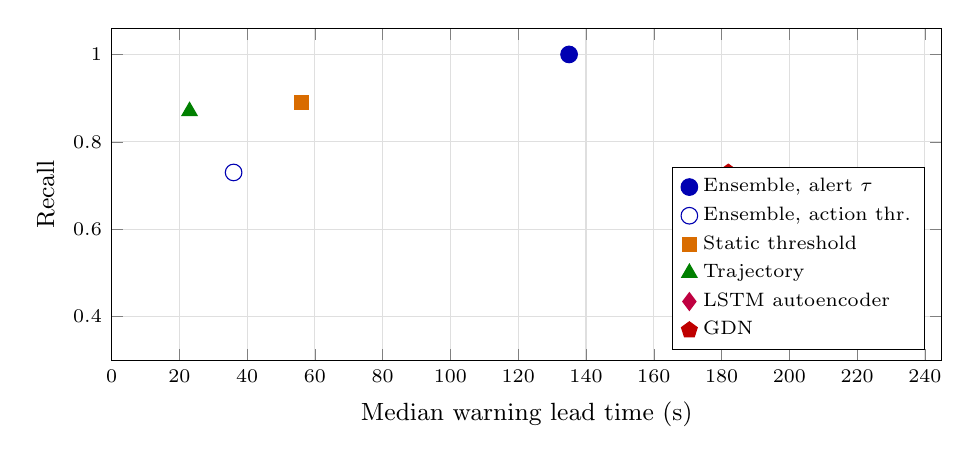
\begin{tikzpicture}
\begin{axis}[
  width=\columnwidth, height=58mm,
  xlabel={Median warning lead time (s)}, ylabel={Recall},
  xmin=0, xmax=245, ymin=0.3, ymax=1.06,
  grid=major, grid style={gray!25},
  legend style={font=\scriptsize, at={(0.98,0.03)}, anchor=south east, cells={anchor=west}},
  tick label style={font=\scriptsize}, label style={font=\small},
]
\addplot[only marks, mark=*, mark size=3pt, blue!70!black] coordinates {(135,1.00)};
\addlegendentry{Ensemble, alert $\tau$}
\addplot[only marks, mark=o, mark size=3pt, blue!70!black] coordinates {(36,0.73)};
\addlegendentry{Ensemble, action thr.}
\addplot[only marks, mark=square*, mark size=2.6pt, orange!85!black] coordinates {(56,0.89)};
\addlegendentry{Static threshold}
\addplot[only marks, mark=triangle*, mark size=3.2pt, green!50!black] coordinates {(23,0.87)};
\addlegendentry{Trajectory}
\addplot[only marks, mark=diamond*, mark size=3.2pt, purple] coordinates {(226,0.41)};
\addlegendentry{LSTM autoencoder}
\addplot[only marks, mark=pentagon*, mark size=3pt, red!75!black] coordinates {(182,0.73)};
\addlegendentry{GDN}
\end{axis}
\end{tikzpicture}
\caption{Operating points on the out-of-distribution split at 0.1\,\% FPR (data of
Table~\ref{tab:detect}). Up and right is better; GDN's point hides 6.5 pre-onset false alarms per
satellite-hour.}
\label{fig:operating}
\end{figure}

\textbf{Two operating points.} The headline uses the alert level $\tau$; the core acts later, at
$\bar p(t,60)\ge 0.5$. Scored at that action threshold the ensemble's recall is 0.73--0.89 with a 36--40\,s
lead (Table~\ref{tab:detect}, second row): CASSANDRA \emph{warns} more than two minutes ahead and
\emph{acts} about half a minute ahead, by design, to avoid acting on low-probability alerts.

\textbf{Per attack type.} Fig.~\ref{fig:bytype} breaks the in-distribution lead down by attack type
(183 failing satellites in 140 attack episodes, recall 1.00 for every type). Slow mechanisms (A3 power
drain, B1 masking) give the longest leads; cross-link propagation (C1) the shortest, because a relayed
command can latch a neighbour's heater within seconds.

\begin{figure}[t]
\centering
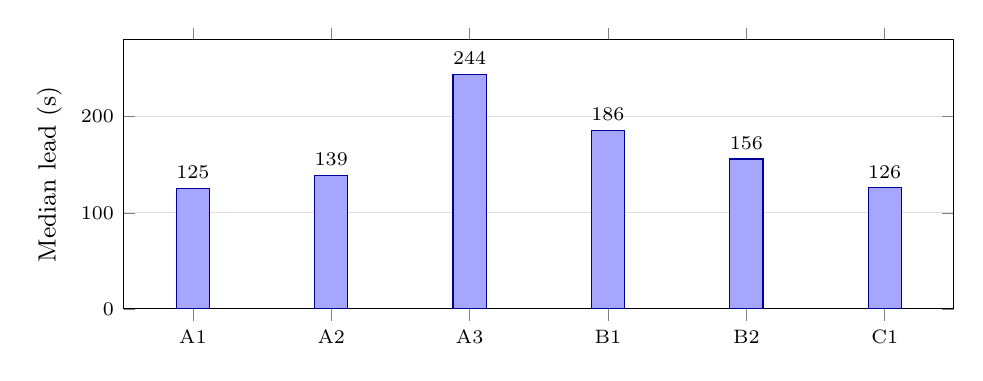
\begin{tikzpicture}
\begin{axis}[
  width=\columnwidth, height=50mm, ybar, bar width=12pt,
  symbolic x coords={A1,A2,A3,B1,B2,C1}, xtick=data,
  ylabel={Median lead (s)}, ymin=0, ymax=280,
  nodes near coords, nodes near coords style={font=\scriptsize},
  tick label style={font=\scriptsize}, label style={font=\small},
  ymajorgrids, grid style={gray!25},
]
\addplot[fill=blue!35, draw=blue!60!black] coordinates {(A1,125) (A2,139) (A3,244) (B1,186) (B2,156) (C1,126)};
\end{axis}
\end{tikzpicture}
\caption{Median lead by attack type, in-distribution split, ensemble at $\tau$ (failing satellites:
A1 28, A2 31, A3 16, B1 15, B2 14, C1 79). Source: \file{results/manifest.json}, \texttt{stress.variants.original}
(\texttt{python -m eval.stress}).}
\label{fig:bytype}
\end{figure}

\subsection{Calibration, attribution and uncertainty heads}
Table~\ref{tab:heads} reports the secondary heads. Calibration error stays below 0.005 at every
horizon on all three splits. The next affected subsystem is predicted well on synthetic noise (top-1
0.83--0.86) but drops to 0.24 under real OPS-SAT noise; attack-versus-fault AUROC is 0.94--0.95.

\begin{table}[t]
\caption{Secondary heads (\file{docs/NUMBERS.md}, \file{results/eval/metrics.json}).}
\label{tab:heads}
\centering
\setlength{\tabcolsep}{4pt}
\begin{tabular}{@{}lccc@{}}
\toprule
Metric & ID & OOD & Real \\
\midrule
ECE, all horizons & $\le$0.005 & $\le$0.005 & $\le$0.005 \\
\quad ID at 10/30/60/120\,s & \multicolumn{3}{l}{0.0007 / 0.0011 / 0.0021 / 0.0034} \\
Next subsystem, top-1 & 0.86 & 0.83 & 0.24 \\
Next subsystem, top-3 & 1.00 & 0.99 & 0.82 \\
Malicious vs fault, AUROC & 0.95 & 0.94 & 0.94 \\
\bottomrule
\end{tabular}
\end{table}

\subsection{Robustness and stress tests}
Under projected-gradient perturbations of the forgeable housekeeping channels (Fig.~\ref{fig:robust};
12 episodes, a small sample, hence the non-monotonic curve) the ensemble's recall stays between 0.75
and 1.00, while the static threshold stays at 0.83. Stress variants that spoof every ground origin or
remove all telecommands leave recall at 1.00 with leads of 133--135\,s: on this benchmark the cyber
features are not what detects (Sec.~\ref{sec:feas}).

\begin{figure}[t]
\centering
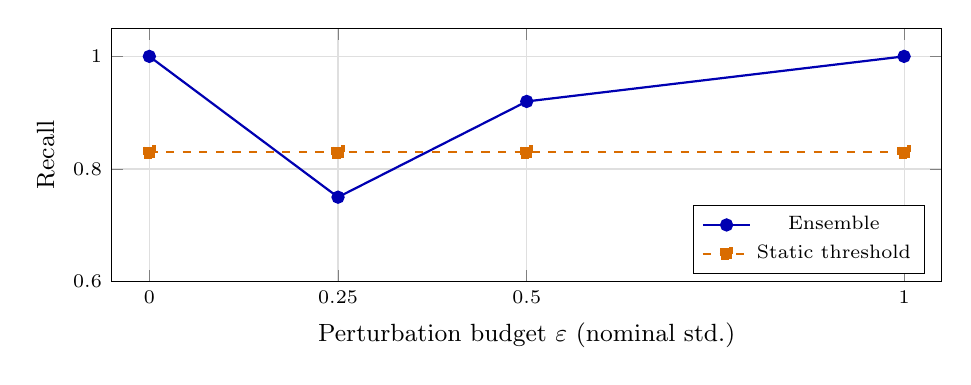
\begin{tikzpicture}
\begin{axis}[
  width=\columnwidth, height=48mm,
  xlabel={Perturbation budget $\varepsilon$ (nominal std.)}, ylabel={Recall},
  xmin=-0.05, xmax=1.05, ymin=0.6, ymax=1.05, xtick={0,0.25,0.5,1.0},
  grid=major, grid style={gray!25},
  legend style={font=\scriptsize, at={(0.98,0.03)}, anchor=south east},
  tick label style={font=\scriptsize}, label style={font=\small},
]
\addplot[thick, blue!70!black, mark=*] coordinates {(0,1.00) (0.25,0.75) (0.5,0.92) (1.0,1.00)};
\addlegendentry{Ensemble}
\addplot[thick, dashed, orange!85!black, mark=square*] coordinates {(0,0.83) (0.25,0.83) (0.5,0.83) (1.0,0.83)};
\addlegendentry{Static threshold}
\end{axis}
\end{tikzpicture}
\caption{Recall under telemetry perturbation (\file{results/eval/robustness.json},
\texttt{python -m eval.robustness --episodes 12}).}
\label{fig:robust}
\end{figure}

\subsection{Closed-loop response (upper bound)}
Re-running 24 test episodes with CASSANDRA acting on the twin (Table~\ref{tab:closed}) averted 13 of the
18 failures that occur without a response, caused no new failure and kept mean availability at 0.9989,
with one false containment (0.05 per orbit) and one gated decision. This is an \emph{upper bound}: the
planner uses the simulator as its own model, which a real system would not have. An earlier figure of
61\,\% from the interim evaluation is not comparable, because that run let the simulator's safe mode
delete commands by their hidden attack label; the fix removed that oracle.

\begin{table}[t]
\caption{Closed loop on the twin, 24 episodes (\file{results/manifest.json}, \texttt{closed\_loop};
\texttt{python -m eval.closed\_loop --episodes 24}). Upper bound.}
\label{tab:closed}
\centering
\footnotesize
\begin{tabular}{@{}lr@{}}
\toprule
Failures averted & 13 / 18 (72.2\,\%; Wilson 49.1--87.5\,\%) \\
New failures caused by a response & 0 \\
Mean availability & 0.9989 \\
False containments & 1 (0.05 per orbit) \\
Actions taken: safe mode / isolate & 13 / 11 \\
Decisions gated by uncertainty & 1 \\
\bottomrule
\end{tabular}
\end{table}

\subsection{Live scenarios with the core in the loop}
Table~\ref{tab:live} summarises the live runs (attack at $t=60$\,s; times are seconds after the attack;
twin limit 45\,\degC). No satellite reached its limit in the runs of the final configuration and no
non-attacked satellite was contained. For A1, $\Jcost$ chooses to cut the heater and keep the satellite
in service (``contains'', not ``quarantines''); repeated commands escalate to safe mode, which refuses
them. The cost term for future relay victims made C1 source containment systematic: from 5 to 6 sources
of 6, from 10 to 6 victims touched, and a median time to contain of 12\,s instead of 57\,s.

\begin{table*}[t]
\caption{Live scenarios, CASSANDRA in closed loop with the twin (simulated) and with the ESP8266 node.
Sources: \file{results/live\_manifest.json} (\texttt{scripts/phase6\_runs.py}),
\file{results/phase6\_block3.json} and \file{results/phase6\_c1\_prefix.json} (C1 before/after),
\file{results/board\_rule\_dryrun.txt}, \file{results/board\_a1.json}.}
\label{tab:live}
\centering
\footnotesize
\setlength{\tabcolsep}{3pt}
\begin{tabular}{@{}p{34mm}p{20mm}p{32mm}p{26mm}p{30mm}p{24mm}@{}}
\toprule
Scenario & Target & First action (by $\Jcost$) & Action at & Max temperature & Outcome \\
\midrule
A1, seeds 1--3 & E, G, J & isolate subsystem (heater cut) & 62 / 116 / 216\,s & 33.7 / 39.6 / 36.5\,\degC & healed \\
A1 re-asserted, seeds 1--3 & E, G, J & safe mode & 43 / 84 / 203\,s & 29.0 / 36.0 / 34.4\,\degC & healed after stop \\
B1 masking, seeds 1--3 & E, G, J & isolate subsystem & 75 / 55 / 75\,s & 36.5 / 32.1 / 25.1\,\degC & healed \\
B1 masking, seeds 4--6 & C, H, L & monitor hit at 8\,s; contained & 66 / 79 / 68\,s & 39.6 / 29.9 / 38.8\,\degC & healed \\
C1 relay, seeds 1--6 (before fix) & sources A, D, K, F, I, L & quarantine of source & 37--137\,s (5/6) & no victim at limit & 10 victims touched \\
C1 relay, seeds 1--6 (final) & same & quarantine of source & 12, 12, 12, 12, 32, 42\,s & no victim at limit & 6 victims touched \\
Clean, seeds 1--3 & --- & none & --- & --- & 0 false containments \\
A1 on node, dry run (firmware model) & B & heater cut, $\hat p(t,30)=0.87$ & $\approx$19\,s & 54.0\,\degC{} (limit 60) & healed at 27.6\,\degC \\
\textbf{A1 on the physical node} & \textbf{B} & \textbf{heater cut} & \textbf{21.9\,s} & \textbf{54.36\,\degC{} (limit 60)} & \textbf{healed at 30.0\,s} \\
\bottomrule
\end{tabular}
\end{table*}

\textbf{The physical node.} Fig.~\ref{fig:board} shows the A1 run on the ESP8266 node (14~Oct; the
temperature is computed by the node's firmware, there is no sensor). The node was flagged 5.9\,s after
the attack command, the heater was cut 21.9\,s after it, and the node was healed at 30.0\,s
(\file{results/board\_a1.json}, times as received by the dashboard). In the bridge log the heater ran for
20.0\,s and the temperature peaked at 54.36\,\degC, 5.6\,\degC{} below the limit. For comparison, the
Phase~2 demonstrator quarantined at 53.3\,\degC{} after 18.8\,s, while a 60\,\degC{} threshold alarm
would have fired at 23.3\,s.

\begin{figure}[t]
\centering
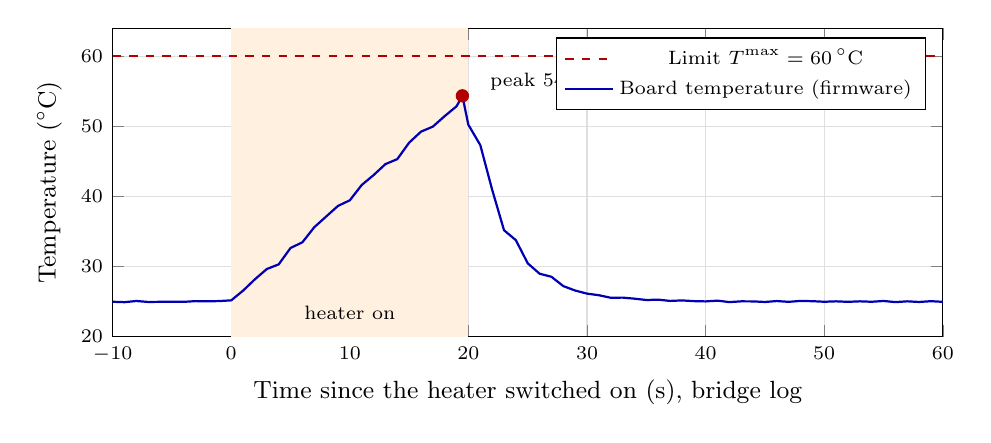
\begin{tikzpicture}
\begin{axis}[
  width=\columnwidth, height=55mm,
  xlabel={Time since the heater switched on (s), bridge log}, ylabel={Temperature (\degC)},
  xmin=-10, xmax=60, ymin=20, ymax=64,
  grid=major, grid style={gray!25},
  legend style={font=\scriptsize, at={(0.98,0.97)}, anchor=north east},
  tick label style={font=\scriptsize}, label style={font=\small},
]
\fill[orange!12] (axis cs:0,20) rectangle (axis cs:19.99,64);
\addplot[thick, red!70!black, dashed, domain=-10:60, samples=2] {60};
\addlegendentry{Limit $T^{\max}=60$\,\degC}
\addplot[thick, blue!70!black] coordinates {
(-10,24.99) (-9,24.93) (-8,25.10) (-7,24.96) (-6,24.98) (-5,24.99) (-4,24.98) (-3,25.08) (-2,25.05)
(-1,25.09) (0,25.19) (1,26.58) (2,28.20) (3,29.66) (4,30.32) (5,32.66) (6,33.47) (7,35.62) (8,37.14)
(9,38.66) (10,39.46) (11,41.64) (12,43.05) (13,44.62) (14,45.33) (15,47.68) (16,49.25) (17,49.97)
(18,51.47) (19,52.87) (19.49,54.36) (19.99,50.24) (21,47.33) (22,40.96) (23,35.19) (24,33.77) (25,30.47)
(26,28.99) (27,28.55) (28,27.22) (29,26.59) (30,26.15) (31,25.92) (32,25.56) (33,25.58) (34,25.43)
(35,25.24) (36,25.29) (37,25.11) (38,25.18) (39,25.08) (40,25.04) (41,25.15) (42,24.94) (43,25.05)
(44,25.04) (45,24.96) (46,25.09) (47,24.98) (48,25.11) (49,25.07) (50,24.99) (51,25.05) (52,24.98)
(53,25.05) (54,24.99) (55,25.10) (56,24.94) (57,25.05) (58,24.96) (59,25.07) (60,24.98)};
\addlegendentry{Board temperature (firmware)}
\addplot[only marks, mark=*, mark size=2.2pt, red!70!black] coordinates {(19.49,54.36)};
\node[font=\scriptsize, anchor=west] at (axis cs:21,56.5) {peak 54.36\,\degC, heater cut};
\node[font=\scriptsize, anchor=south] at (axis cs:10,21) {heater on};
\end{axis}
\end{tikzpicture}
\caption{Attack A1 on the physical ESP8266 node, contained by CASSANDRA (shaded: heater on). One
sample per second from \file{results/board\_a1\_curve.csv} (2\,Hz), plus the exact peak sample;
temperature emulated by the firmware.}
\label{fig:board}
\end{figure}

\subsection{Attack-chain reconstruction and rehearsals}
The incident correlator built a chain in every live run (\file{results/incident\_metrics.json}): A1
3/3 (assembly delay 22, 52, 197\,s after the first observed evidence, i.e.\ the forecaster's warning
time after a legitimate-looking command), B1 3/3 with the deception step (8\,s, the monitor's
confirmation window) and C1 6/6 (0\,s, one victim touched before containment in each run). Two
unattended rehearsals of the full demonstration (\file{results/rehearsal.json}) met every milestone:
node A1 flagged at 5.4--6.1\,s and cut at 21.4--22.1\,s; re-asserted A1 in safe mode at 21.4--22.3\,s;
B1 at 10$\times$ speed caught at 2.9--3.0\,s and contained at 12.6--12.9\,s; C1 source quarantined at
5.7--6.7\,s.

\subsection{Latency}
Table~\ref{tab:latency} gives the measured timings. Inference and live planning fit the 150\,ms budget
on the laptop; the offline evaluator's planner (more candidates, in-process twin copies) does not, and
the Raspberry~Pi target has not been measured.

\begin{table}[t]
\caption{Timing per tick on an x86 laptop (\file{results/manifest.json} \texttt{latency},
\texttt{closed\_loop}; \file{docs/STATUS.md}). Budget: 150\,ms.}
\label{tab:latency}
\centering
\footnotesize
\setlength{\tabcolsep}{4pt}
\begin{tabular}{@{}lr@{}}
\toprule
Ensemble inference, 5 models, 1 thread (median / p95) & 17.6 / 20.9\,ms \\
\quad same, three runs under varying load (median) & 17.6--34.1\,ms \\
Ensemble inference, 4 threads (median / p95) & 21.9 / 40.0\,ms \\
Core tick, live runs (median) & 28--36\,ms \\
Live planning per decision (median) & 61--89\,ms \\
Offline evaluator planning (median / p95) & 254 / 402\,ms \\
\bottomrule
\end{tabular}
\end{table}

% =====================================================================================================
\section{Feasibility, Realism and Space Constraints}
\label{sec:feas}

\textbf{What is real and what is not.} The defence software, the bus, the contract, the twin's physics
and the response loop run end to end, live, and survive unattended rehearsals. The constellation is
simulated; the node's temperature is computed by its firmware; ISL cuts on the node are logical. All
training and evaluation data are synthetic (with real noise in one split); none of the results is a
flight or space-qualified measurement.

\textbf{Saturated benchmark.} Every ablation (single model, no engineered features, unconstrained graph,
no residual) and the stress tests without telecommands also reach recall 1.00 on the synthetic sets
(Table~\ref{tab:detect}). These numbers therefore do not demonstrate the benefit of the graph structure or
of the cyber features; a harder generator (weaker attacks hidden in normal operations, faults that mimic
attacks) is needed for that comparison.

\textbf{Thermal and power.} The twin's thermal model is first-order with a time constant of about
150\,s; at the 30\,s horizon a linear forecast crosses 0.85 only about 4\,s before $T^{\max}$, which is
why the core decides on the 60\,s horizon. Safe mode is a realistic, physically motivated response:
it sheds the heater and refuses re-asserted commands without needing to know they are malicious.

\textbf{Radiation and single-event upsets.} The Theil--Sen trend ignores a single corrupted sample, and
the monitor's frozen-value rule needs a whole window; fault F2 (single-tick upset) triggered no action
in tests. The models are small (42.7\,k parameters per member, about 1.1\,MB for the ensemble), which
eases memory scrubbing, but nothing here has been run on radiation-tolerant hardware.

\textbf{Compute and energy.} Inference takes 17.6\,ms per tick for 12 satellites on one CPU thread of a
laptop. The design places the core on the ground station; an on-board deployment would need the
measurement on an ARM-class processor and an energy budget, which we have not done.

\textbf{Intermittent links.} The ingest stage holds a value for at most 3\,s and then marks it stale;
a watchdog closes ticks when no message arrives; reroutes use only feasible links. The testbed assumes
continuous telemetry; a real ground-segment deployment sees each satellite only during contact windows,
which shortens the usable lead time and argues for an on-board or store-and-forward variant.

\textbf{Adversarial pressure.} The uncertainty gate and the 25\,\% isolation budget limit how far
forged precursors can push the defence into isolating healthy satellites; quarantine requires an
observed cyber cause. The monitor fails, by assumption, if every independent channel of a subsystem is
forged at once. Brief false flags still occur at the low alert level ($\tau\approx 0.015$) without
leading to actions or attack chains.

\textbf{Trade-offs.} Table~\ref{tab:tradeoff} lists the main design choices and their costs.

\begin{table}[t]
\caption{Design trade-offs.}
\label{tab:tradeoff}
\centering
\footnotesize
\setlength{\tabcolsep}{3pt}
\begin{tabular}{@{}p{27mm}p{27mm}p{25mm}@{}}
\toprule
Choice & Gain & Cost \\
\midrule
Alert at $\tau$ (0.1\,\% FPR), act at 0.5 & warn $>$2\,min ahead, act on likely failures & act $\approx$36--40\,s ahead; some misses at the act level \\
Node rule $\hat p(t,30)\ge0.85$ & visible climb, margin as in Phase 2 & 5.6\,\degC{} margin on the node \\
Shadow twin, empty queue & no oracle of attacker intent & assumes observed effects persist \\
Sum of risks in $R$ & spares more satellites & larger state to roll out \\
Ensemble of 5 & uncertainty for the gate & 5$\times$ inference \\
\bottomrule
\end{tabular}
\end{table}

\textbf{Known limits.} CASSANDRA would not have prevented the KA-SAT wiper, which acted in the ground
segment; its 1\,s loop cannot react to microsecond-scale events; it has no lead time against a single
destructive command without precursor.

% =====================================================================================================
\section{Conclusion and Future Work}
\label{sec:conclusion}

CASSANDRA forecasts mission failure instead of scoring anomalies and acts on the forecast with the least
disruptive response that a shadow twin predicts will work. On held-out synthetic scenarios it warned of
every failure more than two minutes ahead at a 0.1\,\% false-positive rate, averted most failures in
closed loop (upper bound), and contained every live attack we ran, including one on a physical node,
before its limit. The prototype is complete: a frozen message contract, a live 12-satellite twin, a
physical node, the defence core with an incident correlator, an operator dashboard and a reproducible
evaluation pipeline.

The evidence is limited by synthetic data, a saturated benchmark and a closed loop that plans with the
simulator itself. Next steps, in order: a harder generator to measure what the graph and the cyber
features contribute; lead-time results on SCAD and false-alarm rates on ESA-ADB; latency and energy on
the Raspberry~Pi and an ARM on-board target; ESP32 nodes with real temperature and current sensors and
radio inter-satellite links; and a planner whose model is learned from telemetry rather than taken from
the simulator.

\section*{Acknowledgment}
The authors thank the organisers and reviewers of the IASTAM~6.0 Technical Challenge.

\bibliographystyle{IEEEtran}
\bibliography{references}

\end{document}
